\documentclass[a4paper, 12pt]{article}
\usepackage{lmodern}
\usepackage{amssymb,amsmath}
\usepackage{ifxetex,ifluatex}
\usepackage{fixltx2e} % provides \textsubscript
\ifnum 0\ifxetex 1\fi\ifluatex 1\fi=0 % if pdftex
  \usepackage[T1]{fontenc}
  \usepackage[utf8]{inputenc}
\else % if luatex or xelatex
  \ifxetex
    \usepackage{mathspec}
  \else
    \usepackage{fontspec}
  \fi
  \defaultfontfeatures{Ligatures=TeX,Scale=MatchLowercase}
\fi
% use upquote if available, for straight quotes in verbatim environments
\IfFileExists{upquote.sty}{\usepackage{upquote}}{}
% use microtype if available
\IfFileExists{microtype.sty}{%
\usepackage{microtype}
\UseMicrotypeSet[protrusion]{basicmath} % disable protrusion for tt fonts
}{}
\usepackage[left=3.5cm,right=2.5cm,top=2.5cm,bottom=2.5cm]{geometry}
\usepackage{hyperref}
\PassOptionsToPackage{usenames,dvipsnames}{color} % color is loaded by hyperref
\hypersetup{unicode=true,
            pdftitle={Crítica à definição de intervalo de confiança, predição e campo de arbítrio na NBR 14.653-02},
            pdfauthor={Luiz Fernando Palin Droubi; Carlos Augusto Zilli; Willian Zonato; Norberto Hochheim},
            colorlinks=true,
            linkcolor=red,
            citecolor=green,
            urlcolor=magenta,
            breaklinks=true}
\urlstyle{same}  % don't use monospace font for urls
\usepackage{longtable,booktabs}
\usepackage{graphicx,grffile}
\makeatletter
\def\maxwidth{\ifdim\Gin@nat@width>\linewidth\linewidth\else\Gin@nat@width\fi}
\def\maxheight{\ifdim\Gin@nat@height>\textheight\textheight\else\Gin@nat@height\fi}
\makeatother
% Scale images if necessary, so that they will not overflow the page
% margins by default, and it is still possible to overwrite the defaults
% using explicit options in \includegraphics[width, height, ...]{}
\setkeys{Gin}{width=\maxwidth,height=\maxheight,keepaspectratio}
\IfFileExists{parskip.sty}{%
\usepackage{parskip}
}{% else
\setlength{\parindent}{0pt}
\setlength{\parskip}{6pt plus 2pt minus 1pt}
}
\setlength{\emergencystretch}{3em}  % prevent overfull lines
\providecommand{\tightlist}{%
  \setlength{\itemsep}{0pt}\setlength{\parskip}{0pt}}
\setcounter{secnumdepth}{5}
% Redefines (sub)paragraphs to behave more like sections
\ifx\paragraph\undefined\else
\let\oldparagraph\paragraph
\renewcommand{\paragraph}[1]{\oldparagraph{#1}\mbox{}}
\fi
\ifx\subparagraph\undefined\else
\let\oldsubparagraph\subparagraph
\renewcommand{\subparagraph}[1]{\oldsubparagraph{#1}\mbox{}}
\fi

%%% Use protect on footnotes to avoid problems with footnotes in titles
\let\rmarkdownfootnote\footnote%
\def\footnote{\protect\rmarkdownfootnote}

%%% Change title format to be more compact
\usepackage{titling}

% Create subtitle command for use in maketitle
\providecommand{\subtitle}[1]{
  \posttitle{
    \begin{center}\large#1\end{center}
    }
}

\setlength{\droptitle}{-2em}

  \title{Crítica à definição de intervalo de confiança, predição e campo de
arbítrio na NBR 14.653-02}
    \pretitle{\vspace{\droptitle}\centering\huge}
  \posttitle{\par}
    \author{Luiz Fernando Palin Droubi\footnote{SPU/SC,
  \href{mailto:luiz.droubi@planejamento.gov.br}{\nolinkurl{luiz.droubi@planejamento.gov.br}}} \\ Carlos Augusto Zilli\footnote{UFSC,
  \href{mailto:carloszilli@gmail.com}{\nolinkurl{carloszilli@gmail.com}}} \\ Willian Zonato\footnote{SPU/SC,
  \href{mailto:willian.zonato@planejamento.gov.br}{\nolinkurl{willian.zonato@planejamento.gov.br}}} \\ Norberto Hochheim\footnote{UFSC,
  \href{mailto:hochheim@gmail.com}{\nolinkurl{hochheim@gmail.com}}}}
    \preauthor{\centering\large\emph}
  \postauthor{\par}
      \predate{\centering\large\emph}
  \postdate{\par}
    \date{02/09/2019}

\usepackage[brazil]{babel}
\usepackage{graphicx}
\usepackage{float}
\usepackage{subfig}
\usepackage{caption}
\usepackage{lastpage}
\usepackage{rotating}
\usepackage{dcolumn}
\setlength{\parindent}{1.25cm} % Default is 15pt.
\usepackage{indentfirst}
\usepackage{fontspec} % para Arial
\setmainfont{Arial}
\newcommand{\pkg}[1]{{\normalfont\fontseries{b}\selectfont #1}}
\let\proglang=\textsf
\let\code=\texttt
\usepackage{fancyhdr}
% Turn on the style
\pagestyle{fancy}
% Clear the header and footer
\fancyhead{}
\fancyfoot{}
% Set the right side of the footer to be the page number
\fancyfoot[R]{\thepage~/~\pageref{LastPage}}
\usepackage{booktabs}
\usepackage{longtable}
\usepackage{array}
\usepackage{multirow}
\usepackage{wrapfig}
\usepackage{float}
\usepackage{colortbl}
\usepackage{pdflscape}
\usepackage{tabu}
\usepackage{threeparttable}
\usepackage{threeparttablex}
\usepackage[normalem]{ulem}
\usepackage{makecell}
\usepackage{xcolor}

\begin{document}
\maketitle

\hypertarget{estudos-de-caso}{%
\section{ESTUDOS DE CASO}\label{estudos-de-caso}}

\hypertarget{dados-reais-de-mercado}{%
\subsection{Dados reais de mercado}\label{dados-reais-de-mercado}}

Neste estudo são utilizados os dados disponíveis em Hochheim
(\protect\hyperlink{ref-hochheim}{2015}, pp. 21--22). O modelo utilizado
também foi o obtido no trabalho citado. Para este estudo de caso foi
utilizado o software R 3.5.1 (R CORE TEAM,
\protect\hyperlink{ref-R}{2019}).

\begin{table}[t]

\caption{\label{tab:coefficients}Coeficientes e estatísticas do modelo adotado.}
\centering
\resizebox{\linewidth}{!}{
\begin{tabular}{lrrrrrll}
\toprule
  & Estimate & CI (lower) & CI (upper) & Std. Error & t value & Pr(>|t|) &    \\
\midrule
\rowcolor{gray!6}  (Intercept) & 13.564 & 13.264 & 13.864 & 0.230 & 58.847 & <0.001 & ***\\
area\_total & 0.001 & 0.001 & 0.002 & 0.000 & 5.113 & <0.001 & ***\\
\rowcolor{gray!6}  quartos & 0.164 & 0.118 & 0.210 & 0.035 & 4.626 & <0.001 & ***\\
suites & 0.061 & 0.017 & 0.105 & 0.034 & 1.810 & 0.078 & .\\
\rowcolor{gray!6}  garagens & 0.209 & 0.165 & 0.252 & 0.033 & 6.247 & <0.001 & ***\\
\addlinespace
log(dist\_b\_mar) & -0.141 & -0.176 & -0.105 & 0.027 & -5.174 & <0.001 & ***\\
\rowcolor{gray!6}  rec(padrao) & -0.563 & -0.700 & -0.426 & 0.105 & -5.360 & <0.001 & ***\\
\bottomrule
\end{tabular}}
\end{table}

Um resumo dos coeficientes e estatísticas do modelo pode ser visto na
tabela \ref{tab:coefficients}.

Como o modelo foi ajustado com a transformação logarítmica natural, os
valores ajustados devem ser retransformados para a escala original. Aqui
se adotará a transformação pela mediana da distribuição lognormal, como
em Hochheim (\protect\hyperlink{ref-hochheim}{2015}).

Na escala log, o valor central obtido foi de 13,7764. Pode-se mostrar
que o erro-padrão do ajuste (\(s.e.(\hat Y)\)) para o bem-avaliando
(obtido de acordo com a expressão
\(\sqrt{x_0'\hat\sigma^2(X'X)^{-1}x_o}\)) é de \(\approx\) 0,0300
(também na escala log). O valor de \(t_{41}^{10\%}\) é \(\approx\)
-1,3025 e \(t_{41}^{10\%}\) é \(\approx\) 1,3025. Substituindo-se nas
expressões abaixo, pode-se calcular os limites do IC para a média, já
que é sabido que o intervalo de confiança @80\% foi cálculado com a
distribuição t com 41 graus de liberdade:

\(\hat Y_{inf} = \hat Y + t_{41}^{10\%}s.e.(\hat Y)\) e
\(\hat Y_{sup} = \hat Y + t_{41}^{90\%}s.e.(\hat Y)\)

Ou seja:

\(\hat Y_{inf} = 13,7764 - 1,3025.0,0300\) e
\(\hat Y_{sup} = 13,7764 + 1,3025.0,0300\)

Caso se opte por arbitrar o valor da estimativa central (R\$961.660,64)
e o intervalo de confiança, a avaliação intervalar fica limitada pelo
último, ou seja, entre R\$924.768,13 e R\$1.000.024,94 e o campo de
arbítrio ({[}R\$817.411,55; R\$1.105.909,74{]}) não pode ser utilizado.

No entanto, caso seja arbitrado o valor de R\$1.100.000,00 para o
bem-avaliando, como em Hochheim (\protect\hyperlink{ref-hochheim}{2015},
pp. 73--74), os novos limites intervalares ficam entre R\$1.060.973,75 e
R\$1.105.909,74.

Transformando-se estes valores para a escala log-natural, tem-se que
13,8747, 13,9108 e 13,9162.

Ora, se sabe-se o valor do erro-padrão naquele ponto e o valor central
do IC, pode-se calcular o valor de t para os novos valores:

\(t_{inf} =\) 3,27\\
\(t_{arbitrado} =\) 4,48\\
\(t_{sup} =\) 4,65

Ora, de posse dos t calculados acima, pode-se calcular as suas
probabilidades de ocorrência: 0,11\%, 0,003\% e 0,0017\%. Ou seja, de
acordo com o IC originalmente calculado, o valor arbitrado, o valor
inferior e o valor calculado tem probabilidade baixíssima de ocorrer.

Isso, contudo, apenas significa que os valores inferior, arbitrado e
superior encontram-se muito acima do intervalo de confiança para a
\emph{média}, ou seja, significa apenas que os valores citados,
``arbitrados'' são superiores à média do mercado.

Se, por outro lado, considera-se o intervalo de predição:

\(\hat Y_{inf} =\) 13,5949 \(\hat Y_{sup} =\) 13,9579

Na escala original, 802.017,63 \(\leq\) 961.660,64 \(\leq\)
1.153.080,88.

Porém, neste caso o IP estaria limitado pelo campo de arbítrio, pois
este está no intervalo {[}R\$817.411,55, R\$1.105.909,74{]}.

Da mesma maneira que foi feito para o IC, pode-se calcular a que
probabilidade está associado o campo de arbítrio em relação ao IP:

\(t_{inf-CA} =\) -1,17\\
\(t_{sup-CA} =\) 1,00

Ou seja, de acordo com o IP, o limite inferior do CA encontra-se no
percentil 12,50\% e o limite superior do CA no percentil 83,90\%, de
maneira que, portanto, o C.A. não pode ser inteiramente utilizado,
apesar de seus limites se encontrarem em percentis confortáveis do IP.

A fórmula para o cálculo do intervalo de predição pode ser escritada
seguinte forma:

\[\hat y_0 \pm t_{n-k}^{\alpha/2}\sqrt{\sigma^2+s.e.^2(\hat y_o)}\]
Deve-se notar que, fixado o valor central \(\hat y_0\) e a amplitude do
intervalo, pode-se calcular o valor do termo
\(\sqrt{\sigma^2+s.e.^2(\hat y_o)}\) em função do \(t\) especificado. No
limite, sabe-se que a distribuição \(t\) aproxima-se assintoticamente da
distribuição normal, que será adotada aqui preliminarmente, por
simplicidade.

\hypertarget{dados-randomicos}{%
\subsection{Dados randômicos}\label{dados-randomicos}}

Imagine-se que em um determinado modelo previamente ajustado, foi
estimado o valor de um bem em R\$1.000.000,00. Imagine-se então que o
modelo possui graus de liberdade suficiente para que o intervalo de
predição possa ser assumido normalmente distribuído. Isto implica que o
termo \(\sqrt{\sigma^2+s.e.^2(\hat y_o)}\) possui os seguintes valores,
dependendo da amplitude do IP calculado:

\begin{longtable}[]{@{}crrrrrr@{}}
\toprule
\begin{minipage}[b]{0.08\columnwidth}\centering
Amplitude IP\strut
\end{minipage} & \begin{minipage}[b]{0.23\columnwidth}\raggedleft
\(\sqrt{\sigma^2+s.e.^2(\hat y_o)}\)\strut
\end{minipage} & \begin{minipage}[b]{0.13\columnwidth}\raggedleft
Semi-amplitude do CA\strut
\end{minipage} & \begin{minipage}[b]{0.09\columnwidth}\raggedleft
\(Z_{inf}\)\strut
\end{minipage} & \begin{minipage}[b]{0.09\columnwidth}\raggedleft
\(Z_{sup}\)\strut
\end{minipage} & \begin{minipage}[b]{0.09\columnwidth}\raggedleft
\(p_{inf}\)\strut
\end{minipage} & \begin{minipage}[b]{0.09\columnwidth}\raggedleft
\(p_{sup}\)\strut
\end{minipage}\tabularnewline
\midrule
\endhead
\begin{minipage}[t]{0.08\columnwidth}\centering
30\%\strut
\end{minipage} & \begin{minipage}[t]{0.23\columnwidth}\raggedleft
117.045,62\strut
\end{minipage} & \begin{minipage}[t]{0.13\columnwidth}\raggedleft
150.000\strut
\end{minipage} & \begin{minipage}[t]{0.09\columnwidth}\raggedleft
-1,28\strut
\end{minipage} & \begin{minipage}[t]{0.09\columnwidth}\raggedleft
1,28\strut
\end{minipage} & \begin{minipage}[t]{0.09\columnwidth}\raggedleft
10,00\%\strut
\end{minipage} & \begin{minipage}[t]{0.09\columnwidth}\raggedleft
90,00\%\strut
\end{minipage}\tabularnewline
\begin{minipage}[t]{0.08\columnwidth}\centering
40\%\strut
\end{minipage} & \begin{minipage}[t]{0.23\columnwidth}\raggedleft
156.060,83\strut
\end{minipage} & \begin{minipage}[t]{0.13\columnwidth}\raggedleft
150.000\strut
\end{minipage} & \begin{minipage}[t]{0.09\columnwidth}\raggedleft
-0,96\strut
\end{minipage} & \begin{minipage}[t]{0.09\columnwidth}\raggedleft
0,96\strut
\end{minipage} & \begin{minipage}[t]{0.09\columnwidth}\raggedleft
16,80\%\strut
\end{minipage} & \begin{minipage}[t]{0.09\columnwidth}\raggedleft
83,20\%\strut
\end{minipage}\tabularnewline
\begin{minipage}[t]{0.08\columnwidth}\centering
50\%\strut
\end{minipage} & \begin{minipage}[t]{0.23\columnwidth}\raggedleft
195.076,04\strut
\end{minipage} & \begin{minipage}[t]{0.13\columnwidth}\raggedleft
150.000\strut
\end{minipage} & \begin{minipage}[t]{0.09\columnwidth}\raggedleft
-0,77\strut
\end{minipage} & \begin{minipage}[t]{0.09\columnwidth}\raggedleft
0,77\strut
\end{minipage} & \begin{minipage}[t]{0.09\columnwidth}\raggedleft
22,10\%\strut
\end{minipage} & \begin{minipage}[t]{0.09\columnwidth}\raggedleft
77,90\%\strut
\end{minipage}\tabularnewline
\bottomrule
\end{longtable}

O mesmo pode ser feito para a distribuição t com 40 graus de liberdade,
por exemplo:

\begin{longtable}[]{@{}crrrrrr@{}}
\toprule
\begin{minipage}[b]{0.08\columnwidth}\centering
Amplitude IP\strut
\end{minipage} & \begin{minipage}[b]{0.22\columnwidth}\raggedleft
\(\sqrt{\sigma^2+s.e.^2(\hat y_o)}\)\strut
\end{minipage} & \begin{minipage}[b]{0.13\columnwidth}\raggedleft
Semi-amplitude do CA\strut
\end{minipage} & \begin{minipage}[b]{0.09\columnwidth}\raggedleft
\(t_{inf}\)\strut
\end{minipage} & \begin{minipage}[b]{0.09\columnwidth}\raggedleft
\(t_{sup}\)\strut
\end{minipage} & \begin{minipage}[b]{0.12\columnwidth}\raggedleft
\(p_{inf}\)\strut
\end{minipage} & \begin{minipage}[b]{0.09\columnwidth}\raggedleft
\(p_{sup}\)\strut
\end{minipage}\tabularnewline
\midrule
\endhead
\begin{minipage}[t]{0.08\columnwidth}\centering
30\%\strut
\end{minipage} & \begin{minipage}[t]{0.22\columnwidth}\raggedleft
115.112,15\strut
\end{minipage} & \begin{minipage}[t]{0.13\columnwidth}\raggedleft
150.000\strut
\end{minipage} & \begin{minipage}[t]{0.09\columnwidth}\raggedleft
-1,30\strut
\end{minipage} & \begin{minipage}[t]{0.09\columnwidth}\raggedleft
1,30\strut
\end{minipage} & \begin{minipage}[t]{0.12\columnwidth}\raggedleft
10,00\%\strut
\end{minipage} & \begin{minipage}[t]{0.09\columnwidth}\raggedleft
90,00\%\strut
\end{minipage}\tabularnewline
\begin{minipage}[t]{0.08\columnwidth}\centering
40\%\strut
\end{minipage} & \begin{minipage}[t]{0.22\columnwidth}\raggedleft
153.482,87\strut
\end{minipage} & \begin{minipage}[t]{0.13\columnwidth}\raggedleft
150.000\strut
\end{minipage} & \begin{minipage}[t]{0.09\columnwidth}\raggedleft
-0,98\strut
\end{minipage} & \begin{minipage}[t]{0.09\columnwidth}\raggedleft
0,98\strut
\end{minipage} & \begin{minipage}[t]{0.12\columnwidth}\raggedleft
16,70\%\strut
\end{minipage} & \begin{minipage}[t]{0.09\columnwidth}\raggedleft
83,30\%\strut
\end{minipage}\tabularnewline
\begin{minipage}[t]{0.08\columnwidth}\centering
50\%\strut
\end{minipage} & \begin{minipage}[t]{0.22\columnwidth}\raggedleft
191.853,58\strut
\end{minipage} & \begin{minipage}[t]{0.13\columnwidth}\raggedleft
150.000\strut
\end{minipage} & \begin{minipage}[t]{0.09\columnwidth}\raggedleft
-0,78\strut
\end{minipage} & \begin{minipage}[t]{0.09\columnwidth}\raggedleft
0,78\strut
\end{minipage} & \begin{minipage}[t]{0.12\columnwidth}\raggedleft
21,90\%\strut
\end{minipage} & \begin{minipage}[t]{0.09\columnwidth}\raggedleft
78,10\%\strut
\end{minipage}\tabularnewline
\bottomrule
\end{longtable}

Ou ainda com 10 graus de liberdade:

\begin{longtable}[]{@{}crrrrrr@{}}
\toprule
\begin{minipage}[b]{0.08\columnwidth}\centering
Amplitude IP\strut
\end{minipage} & \begin{minipage}[b]{0.22\columnwidth}\raggedleft
\(\sqrt{\sigma^2+s.e.^2(\hat y_o)}\)\strut
\end{minipage} & \begin{minipage}[b]{0.13\columnwidth}\raggedleft
Semi-amplitude do CA\strut
\end{minipage} & \begin{minipage}[b]{0.12\columnwidth}\raggedleft
\(t_{inf}\)\strut
\end{minipage} & \begin{minipage}[b]{0.09\columnwidth}\raggedleft
\(t_{sup}\)\strut
\end{minipage} & \begin{minipage}[b]{0.09\columnwidth}\raggedleft
\(p_{inf}\)\strut
\end{minipage} & \begin{minipage}[b]{0.09\columnwidth}\raggedleft
\(p_{sup}\)\strut
\end{minipage}\tabularnewline
\midrule
\endhead
\begin{minipage}[t]{0.08\columnwidth}\centering
30\%\strut
\end{minipage} & \begin{minipage}[t]{0.22\columnwidth}\raggedleft
109.314,81\strut
\end{minipage} & \begin{minipage}[t]{0.13\columnwidth}\raggedleft
150.000\strut
\end{minipage} & \begin{minipage}[t]{0.12\columnwidth}\raggedleft
-1,37\strut
\end{minipage} & \begin{minipage}[t]{0.09\columnwidth}\raggedleft
1,37\strut
\end{minipage} & \begin{minipage}[t]{0.09\columnwidth}\raggedleft
10,00\%\strut
\end{minipage} & \begin{minipage}[t]{0.09\columnwidth}\raggedleft
90,00\%\strut
\end{minipage}\tabularnewline
\begin{minipage}[t]{0.08\columnwidth}\centering
40\%\strut
\end{minipage} & \begin{minipage}[t]{0.22\columnwidth}\raggedleft
145.753,09\strut
\end{minipage} & \begin{minipage}[t]{0.13\columnwidth}\raggedleft
150.000\strut
\end{minipage} & \begin{minipage}[t]{0.12\columnwidth}\raggedleft
-1,03\strut
\end{minipage} & \begin{minipage}[t]{0.09\columnwidth}\raggedleft
1,03\strut
\end{minipage} & \begin{minipage}[t]{0.09\columnwidth}\raggedleft
16,40\%\strut
\end{minipage} & \begin{minipage}[t]{0.09\columnwidth}\raggedleft
83,60\%\strut
\end{minipage}\tabularnewline
\begin{minipage}[t]{0.08\columnwidth}\centering
50\%\strut
\end{minipage} & \begin{minipage}[t]{0.22\columnwidth}\raggedleft
182.191,36\strut
\end{minipage} & \begin{minipage}[t]{0.13\columnwidth}\raggedleft
150.000\strut
\end{minipage} & \begin{minipage}[t]{0.12\columnwidth}\raggedleft
-0,82\strut
\end{minipage} & \begin{minipage}[t]{0.09\columnwidth}\raggedleft
0,82\strut
\end{minipage} & \begin{minipage}[t]{0.09\columnwidth}\raggedleft
21,50\%\strut
\end{minipage} & \begin{minipage}[t]{0.09\columnwidth}\raggedleft
78,50\%\strut
\end{minipage}\tabularnewline
\bottomrule
\end{longtable}

Pode-se notar nas tabelas acima que a influência do número de graus de
liberdade existe, mas é moderada, caso \((T-k) \geq 10\). Em todos os
casos, a variação mais relevante é a das diferentes amplitudes dos
intervalos de predição, \emph{i.e.}, importa mais a variabilidade
populacional.

Já o impacto da variabilidade do mercado pode ser vista graficamente na
figura \ref{fig:CAs}, onde os pontos e a linha em vermelho representam o
valor ajustado e os limites do Campo de Arbítrio, a área em azul claro
representa o intervalo de predição @ 80\%, a reta azul é a reta de
regressão em relação aos dados amostrais e, finalmente, a área cinza
representa o intervalo de confiança para esta regressão, para vários
cenários hipotéticos.

Primeiramente, foi imaginado um cenário hipotético de mercado
equilibrado, onde, por acaso, o Campo de Arbítrio se ajusta
perfeitamente à variabilidade do mercado e poderia ser utilizado sem
restrições. No segundo cenário, apenas foi considerado um intervalo mais
amplo de validade para o modelo, porém com mesma variabilidade. No
terceiro cenário, chamado de ``Parado'', foi considerado um mercado com
baixíssima variabilidade, para ilustrar o fato que, nestes casos, o
Campo de Arbítrio pode superar os limites populacionais em ambos os
sentidos. Finalmente, no quarto cenário, foi imaginado um mercado
aquecido, com alta variabilidade, onde os limites do Campo de Arbítrio
de \(\pm\) 15\% não chegam nem à metade do intervalo de predição.

\begin{figure}[H]

{\centering 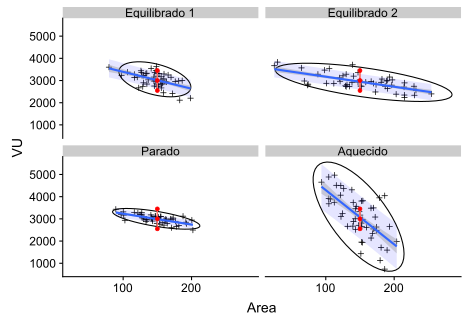
\includegraphics[width=0.95\linewidth]{images/CAs-1} 

}

\caption{Comparação do campo de arbítrio em diferentes realidades mercadológicas.}\label{fig:CAs}
\end{figure}

Como se pode notar, é possível que o campo de arbítrio seja um bom
parâmetro para o arbítrio do valor de mercado de um imóvel, porém isso
só ocorrerá se, por acaso, a variabilidade do mercado for da mesma
magnitude da amplitude do campo de arbítrio.

Se, contudo, o mercado tiver menos variabilidade a utilização dos
limites do C.A. estará sub ou superavaliando o bem-avaliando para aquele
mercado. Já no caso de um mercado com maior variabilidade, a utilização
dos limites do C.A. pode ser insuficiente para dar ao avaliador a
possibilidade de arbitrar valores nas faixas mais distantes da média do
mercado, apesar destes imóveis serem parte da realidade do mercado.

Os coeficientes de determinação dos vários cenários estudados podem ser
vistos na tabela abaixo:

\begin{longtable}[]{@{}lr@{}}
\toprule
Cenário & \(R^2\)\tabularnewline
\midrule
\endhead
Equilíbrio 1 & 0,31\tabularnewline
Equilíbrio 2 & 0,33\tabularnewline
Parado & 0,34\tabularnewline
Aquecido & 0,29\tabularnewline
\bottomrule
\end{longtable}

A tabela abaixo mostra com mais precisão a magnitude do problema:
efetuou-se a estimativa para os valores centrais (\(Area = 150m^2\)) com
o intervalo de predição @80\%. Nos dois primeiros cenários, os limites
do IP e do CA são praticamente equivalentes. Porém, no terceiro cenário
o campo de arbítrio ficaria muito além do IP, enquanto no quarto cenário
o mesmo seria insuficiente para chegar aos extremos do mesmo, pois
estaria limitado pelo IP.

\begin{longtable}[]{@{}lrrrrrr@{}}
\toprule
\begin{minipage}[b]{0.07\columnwidth}\raggedright
Cenário\strut
\end{minipage} & \begin{minipage}[b]{0.13\columnwidth}\raggedleft
Estimativa Central\strut
\end{minipage} & \begin{minipage}[b]{0.13\columnwidth}\raggedleft
\(IP_{inf}\)\strut
\end{minipage} & \begin{minipage}[b]{0.13\columnwidth}\raggedleft
\(IP_{sup}\)\strut
\end{minipage} & \begin{minipage}[b]{0.16\columnwidth}\raggedleft
Amplitude\strut
\end{minipage} & \begin{minipage}[b]{0.09\columnwidth}\raggedleft
\(p_{CA - inf}\)\strut
\end{minipage} & \begin{minipage}[b]{0.09\columnwidth}\raggedleft
\(p_{CA - sup}\)\strut
\end{minipage}\tabularnewline
\midrule
\endhead
\begin{minipage}[t]{0.07\columnwidth}\raggedright
Eq. 1\strut
\end{minipage} & \begin{minipage}[t]{0.13\columnwidth}\raggedleft
3.002,75\strut
\end{minipage} & \begin{minipage}[t]{0.13\columnwidth}\raggedleft
2.603,39\strut
\end{minipage} & \begin{minipage}[t]{0.13\columnwidth}\raggedleft
3.402,11\strut
\end{minipage} & \begin{minipage}[t]{0.16\columnwidth}\raggedleft
26,60\%\strut
\end{minipage} & \begin{minipage}[t]{0.09\columnwidth}\raggedleft
7,43\%\strut
\end{minipage} & \begin{minipage}[t]{0.09\columnwidth}\raggedleft
92,60\%\strut
\end{minipage}\tabularnewline
\begin{minipage}[t]{0.07\columnwidth}\raggedright
Eq. 2\strut
\end{minipage} & \begin{minipage}[t]{0.13\columnwidth}\raggedleft
3.007,71\strut
\end{minipage} & \begin{minipage}[t]{0.13\columnwidth}\raggedleft
2.554,64\strut
\end{minipage} & \begin{minipage}[t]{0.13\columnwidth}\raggedleft
3.460,79\strut
\end{minipage} & \begin{minipage}[t]{0.16\columnwidth}\raggedleft
30,10\%\strut
\end{minipage} & \begin{minipage}[t]{0.09\columnwidth}\raggedleft
10,10\%\strut
\end{minipage} & \begin{minipage}[t]{0.09\columnwidth}\raggedleft
89,90\%\strut
\end{minipage}\tabularnewline
\begin{minipage}[t]{0.07\columnwidth}\raggedright
Parado\strut
\end{minipage} & \begin{minipage}[t]{0.13\columnwidth}\raggedleft
3.008,04\strut
\end{minipage} & \begin{minipage}[t]{0.13\columnwidth}\raggedleft
2.812,56\strut
\end{minipage} & \begin{minipage}[t]{0.13\columnwidth}\raggedleft
3.203,52\strut
\end{minipage} & \begin{minipage}[t]{0.16\columnwidth}\raggedleft
13,00\%\strut
\end{minipage} & \begin{minipage}[t]{0.09\columnwidth}\raggedleft
0,17\%\strut
\end{minipage} & \begin{minipage}[t]{0.09\columnwidth}\raggedleft
99,80\%\strut
\end{minipage}\tabularnewline
\begin{minipage}[t]{0.07\columnwidth}\raggedright
Aquecido\strut
\end{minipage} & \begin{minipage}[t]{0.13\columnwidth}\raggedleft
3.010,51\strut
\end{minipage} & \begin{minipage}[t]{0.13\columnwidth}\raggedleft
1.931,82\strut
\end{minipage} & \begin{minipage}[t]{0.13\columnwidth}\raggedleft
4.089,19\strut
\end{minipage} & \begin{minipage}[t]{0.16\columnwidth}\raggedleft
71,70\%\strut
\end{minipage} & \begin{minipage}[t]{0.09\columnwidth}\raggedleft
29,50\%\strut
\end{minipage} & \begin{minipage}[t]{0.09\columnwidth}\raggedleft
70,50\%\strut
\end{minipage}\tabularnewline
\bottomrule
\end{longtable}

Finalmente, para averiguar a pertinência da adoção do IC para a
avaliação intervalar e para a aferição do Grau de Precisão, foi
elaborada a tabela abaixo:

\begin{longtable}[]{@{}lrrrrrr@{}}
\toprule
\begin{minipage}[b]{0.07\columnwidth}\raggedright
Cenário\strut
\end{minipage} & \begin{minipage}[b]{0.13\columnwidth}\raggedleft
Estimativa Central\strut
\end{minipage} & \begin{minipage}[b]{0.13\columnwidth}\raggedleft
\(IC_{inf}\)\strut
\end{minipage} & \begin{minipage}[b]{0.13\columnwidth}\raggedleft
\(IC_{sup}\)\strut
\end{minipage} & \begin{minipage}[b]{0.16\columnwidth}\raggedleft
Amplitude\strut
\end{minipage} & \begin{minipage}[b]{0.09\columnwidth}\raggedleft
\(p_{CA - inf}\)\strut
\end{minipage} & \begin{minipage}[b]{0.09\columnwidth}\raggedleft
\(p_{CA - sup}\)\strut
\end{minipage}\tabularnewline
\midrule
\endhead
\begin{minipage}[t]{0.07\columnwidth}\raggedright
Equilíbrio 1\strut
\end{minipage} & \begin{minipage}[t]{0.13\columnwidth}\raggedleft
3.002,75\strut
\end{minipage} & \begin{minipage}[t]{0.13\columnwidth}\raggedleft
2.974,54\strut
\end{minipage} & \begin{minipage}[t]{0.13\columnwidth}\raggedleft
3.030,96\strut
\end{minipage} & \begin{minipage}[t]{0.16\columnwidth}\raggedleft
1,88\%\strut
\end{minipage} & \begin{minipage}[t]{0.09\columnwidth}\raggedleft
0,00\%\strut
\end{minipage} & \begin{minipage}[t]{0.09\columnwidth}\raggedleft
100,00\%\strut
\end{minipage}\tabularnewline
\begin{minipage}[t]{0.07\columnwidth}\raggedright
Equilíbrio 2\strut
\end{minipage} & \begin{minipage}[t]{0.13\columnwidth}\raggedleft
3.007,71\strut
\end{minipage} & \begin{minipage}[t]{0.13\columnwidth}\raggedleft
2.975,60\strut
\end{minipage} & \begin{minipage}[t]{0.13\columnwidth}\raggedleft
3.039,82\strut
\end{minipage} & \begin{minipage}[t]{0.16\columnwidth}\raggedleft
2,14\%\strut
\end{minipage} & \begin{minipage}[t]{0.09\columnwidth}\raggedleft
0,00\%\strut
\end{minipage} & \begin{minipage}[t]{0.09\columnwidth}\raggedleft
100,00\%\strut
\end{minipage}\tabularnewline
\begin{minipage}[t]{0.07\columnwidth}\raggedright
Parado\strut
\end{minipage} & \begin{minipage}[t]{0.13\columnwidth}\raggedleft
3.008,04\strut
\end{minipage} & \begin{minipage}[t]{0.13\columnwidth}\raggedleft
2.994,23\strut
\end{minipage} & \begin{minipage}[t]{0.13\columnwidth}\raggedleft
3.021,85\strut
\end{minipage} & \begin{minipage}[t]{0.16\columnwidth}\raggedleft
0,92\%\strut
\end{minipage} & \begin{minipage}[t]{0.09\columnwidth}\raggedleft
0,00\%\strut
\end{minipage} & \begin{minipage}[t]{0.09\columnwidth}\raggedleft
100,00\%\strut
\end{minipage}\tabularnewline
\begin{minipage}[t]{0.07\columnwidth}\raggedright
Aquecido\strut
\end{minipage} & \begin{minipage}[t]{0.13\columnwidth}\raggedleft
3.010,51\strut
\end{minipage} & \begin{minipage}[t]{0.13\columnwidth}\raggedleft
2.934,35\strut
\end{minipage} & \begin{minipage}[t]{0.13\columnwidth}\raggedleft
3.086,67\strut
\end{minipage} & \begin{minipage}[t]{0.16\columnwidth}\raggedleft
5,06\%\strut
\end{minipage} & \begin{minipage}[t]{0.09\columnwidth}\raggedleft
0,00000000005\%\strut
\end{minipage} & \begin{minipage}[t]{0.09\columnwidth}\raggedleft
100,00\%\strut
\end{minipage}\tabularnewline
\bottomrule
\end{longtable}

Como se pode notar, em nenhum dos cenários o Campo de Arbítrio seria
menos restritivo do que o IC, mesmo no cenário de Mercado Aquecido. A
probabilidade de ocorrência de que os limites inferior e superior do
campo de arbítrio estejam dentro do intervalo de confiança para a média
é praticamente zero.

\hypertarget{dados-lognormais}{%
\subsection{Dados lognormais}\label{dados-lognormais}}

Imagine-se um modelo de regressão linear onde a variável resposta tenha
sido transformada com a função logarítmo natural e que, com este modelo,
tenham sido obtidas as seguintes estimativas para o bem avaliando:

\[ln(\hat{Y}) =\]13,8155

\[\hat\sigma =\]0,1003

Então, com este modelo, o avaliador teria obtido os seguintes valores
com o seu software de avaliação:

\begin{longtable}[]{@{}lrrr@{}}
\toprule
CA/IP & Moda & Mediana & Média\tabularnewline
\midrule
\endhead
& 990.000,00 & 1.000.000,00 & 1.005.037,82\tabularnewline
\(CA_{inf}\) & 841.500,00 & 850.000,00 & 854.282,14\tabularnewline
\(CA_{sup}\) & 1.138.500,00 & 1.150.000,00 & 1.155.793,49\tabularnewline
\(IP_{inf}\) & 870.639,20 & 879.433,53 & 883.863,96\tabularnewline
\(IP_{sup}\) & 1.125.724,64 & 1.137.095,60 & 1.142.824,08\tabularnewline
\bottomrule
\end{longtable}

Por simplicidade, aqui foi admitido que o erro na estimativa de
\(\hat{y}\) é zero (\(se(\hat y) = 0\)). Com esta hipótese, o cálculo do
Intervalo de Predição ficou resumido a:

\[IP = \hat{Y} \pm Z_{90}\hat{\sigma}\] Pode ser calculado a que
percentil da distribuição lognormal corresponde cada valor adotado. Oos
resultados podem ser vistos na tabela abaixo:

\begin{longtable}[]{@{}lrrr@{}}
\toprule
CA/IP & Moda & Mediana & Média\tabularnewline
\midrule
\endhead
& 46,00\% & 50,00\% & 52,00\%\tabularnewline
\(CA_{inf}\) & 4,26\% & 5,25\% & 5,81\%\tabularnewline
\(CA_{sup}\) & 90,20\% & 91,80\% & 92,60\%\tabularnewline
\(IP_{inf}\) & 8,35\% & 10,00\% & 10,90\%\tabularnewline
\(IP_{sup}\) & 88,10\% & 90,00\% & 90,90\%\tabularnewline
\bottomrule
\end{longtable}

Pode-se notar que a adoção da estimativa pela moda e do CA inferior
corresponde ao percentil 4,26\%, ou seja, um percentil muito baixo da
distribuição encontrada pelo modelo.

No outro extremo, está a adoção do limite superior do CA e da estimativa
pela média, encontrando-se num percentil extremamente alto da
distribuição encontrada (92,60\%).

Mesmo para a mediana, neste caso, a utilização dos valores extremos do
CA leva a percentis muito extremos da distribuição de probabilidades
(5,25\% e 91,80\%).

Enquanto isto, a adoção da estimativa pela mediana e a utilização do IP
leva aos percentis que consideram-se adequados, ou seja, os percentis
10\% e 90\%.

\hypertarget{avaliacao-intervalar-segundo-a-atual-nbr14.653-02}{%
\subsubsection{Avaliação Intervalar segundo a atual
NBR14.653-02}\label{avaliacao-intervalar-segundo-a-atual-nbr14.653-02}}

Segundo a atual NBR14.653-02, o avaliador teria várias alternativas para
a definição da estimativa final, dentre as quais elencam-se:

\begin{enumerate}
\def\labelenumi{\arabic{enumi}.}
\tightlist
\item
  Adoção da estimativa pela moda e do limite inferior do CA:
\end{enumerate}

Se o avaliador optasse pela moda, adotando o limite inferior do CA, o
intervalo final da avaliação, segundo a atual normativa, seria:
{[}841.500,00; 977.224,64{]}. Ou seja, fazendo-se esta escolha, o
intervalo final obtido estaria entre os percentis 4,26\% e 40,90\%.

\begin{enumerate}
\def\labelenumi{\arabic{enumi}.}
\setcounter{enumi}{1}
\tightlist
\item
  Adoção da mediana, com limite inferior do CA:
\end{enumerate}

Se o avaliador adotasse a mediana como estimativa de tendência central
(lembre-se que para o cálculo da mediana não se utiliza o valor de
\(\hat \sigma\)), e o limite inferior do CA, o avaliador teria como
intervalo final: {[}850.000,00; 987.095,60{]}. Ou seja, fazendo-se esta
escolha, o intervalo final obtido estaria entre os percentis 5,25\% e
44,80\%.

\begin{enumerate}
\def\labelenumi{\arabic{enumi}.}
\setcounter{enumi}{2}
\tightlist
\item
  Simples adoção da mediana:
\end{enumerate}

Se o avaliador adotasse simplesmente a mediana, teria como intervalo
final da avaliação: {[}879.433,53, 1.137.095,60{]}. Ou seja, fazendo-se
esta escolha, o intervalo final obtido estaria entre os percentis 5,25\%
e 91,80\%.

\begin{enumerate}
\def\labelenumi{\arabic{enumi}.}
\setcounter{enumi}{3}
\tightlist
\item
  Adoção da mediana, com limite superior do CA:
\end{enumerate}

Se o avaliador adotasse a mediana como estimativa de tendência central e
o limite superior do CA, o avaliador teria como intervalo final:
{[}1.029.433,53; 1.150.000,00{]}. Ou seja, fazendo-se esta escolha, o
intervalo final obtido estaria entre os percentis 61,40\% e 91,80\%.

\begin{enumerate}
\def\labelenumi{\arabic{enumi}.}
\setcounter{enumi}{4}
\tightlist
\item
  Adoção da média, com limite superior do CA:
\end{enumerate}

Finalmente, se o avaliador optasse pela média e o intervalo superior do
CA, ele teria como intervalo final: {[}1.034.619,63; 1.155.793,49{]}. Ou
seja, fazendo-se esta escolha, o intervalo final obtido estaria entre os
percentis 63,30\% e 92,60\%.

\hypertarget{conclusao}{%
\section{CONCLUSÃO}\label{conclusao}}

A NBR14.653-01 (\protect\hyperlink{ref-NBR1465301}{2001}) e NBR14.653-02
(\protect\hyperlink{ref-NBR1465302}{2011}) fariam melhor em definir
valor médio (\(\mu(Y| X= t)\)), intervalo de confiança para a média
(\(IC(\mu(t)\)), valo.r arbitrado (\(\hat Y\)) e intervalo de predição
para os valores arbitrados.

O avaliador deveria ter o poder de arbitrar valores para os
bem-avaliandos dentro do intervalo de predição! Claro, pois o intervalo
de confiança é para a média, mas o avaliador deveria ter condições de
dizer se o bem-avaliando encontra-se acima ou abaixo dela. Por outro
lado, o avaliador nunca deveria ter o poder de arbitrar valores para a
média fora do IC! Isto é absurdo, pois foi feito uma inferência para a
estimação da média e seu intervalo de confiança, mas a NBR14.653-2
permite ao avaliador arbitrar que a média encontra-se fora do IC! Isto
não faz qualquer sentido científico.

O Campo de Arbítrio do avaliador não é um bom parâmetro para a
arbitragem de valores, dado que o mesmo é constante (\(\pm\) 15\%),
independente da variabilidade do mercado. Ora, como se mostrou no estudo
de caso, com um modelo muito bem ajustado, causa espécie que o valor do
CA fique restrito aos percentis 12,50\% e 83,90\% do IP. Desta maneira
se está restringindo desnecessariamente o avaliador naquele intervalo,
sendo que o avaliador poderia ter maior flexibilidade. Imagine-se o caso
de um modelo menos ajustado, onde o IP seja de aproximadamente 50\%:
pode ocorrer de o C.A. ficar entre percentis muito próximos à média, ou
seja, sabendo-se que há uma grande variabilidade no mercado,
restringe-se o avaliador àqueles 15\%, que muitas vezes é pouco. Por que
não se restringir o avaliador aos percentis 10\% e 90\% do IP?

A NBR14.653-02 tem um problema conceitual: ela mistura o conceito de
valor médio e intervalo de confiança para a média, com o conceito de
valor ajustado e intervalo de predição.

O valor médio e o intervalo de confiança para a média é de pouco
interesse para o avaliador: estes conceitos tem valor mais explicativo.
Pode-se utilizar o valor médio e seu intervalo de confiança para
responder a seguinte pergunta: qual o valor médio de um apartamento com
tais características naquele mercado? Para responder a esta pergunta de
uma maneira qualitativa, deve-se utilizar o conceito de intervalo de
confiança: um apartamento com tais características, naquela localidade,
vale em média R\$3.000,00/m2 \(\pm\) R\$500,00 ao nível de confiança de
80\%. A simples resposta que um apartamento de tais características vale
em média R\$3.000,00/m2 não é uma boa resposta, pois não descreve a
variabilidade do mercado. O IC dá uma idéia da variabilidade em torno da
média.

Existem vários ramos da ciência que se valem destes conceitos, como é o
caso da medicina: ``o modelo comprovou que pessoas com IMC entre 25 e 30
vivem em média 10 anos a mais do que pessoas com IMC\textgreater{}35, ao
nível de 90\%''. Apesar de ser uma média para a população, dificilmente
alguém poderia dizer quantos anos viverá uma determinada pessao com IMC
igual ou superior a 35, contudo, pois a variabilidade é muito maior.

Na Engenharia de Avaliações, contudo, apenas raramente se está
interessado nestas funções descritivas da inferência clássica. Mais
frequentemente se está interessado em conhecer, à partir de uma amostra,
o valor para um novo elemento do mercado, não o valor médio do mercado
de bens com aquelas características. Por isso o avaliador é obrigado a
fazer uma vistoria no bem-avaliando, já que então ele pode intuir se o
imóvel estará acima ou abaixo da média para aquele mercado. Se fosse de
outra maneira, não seria necessário ao avaliador realizar a vistoria,
bastaria ele dizer que em média tal imóvel vale R\$3.000,00 o metro
quadrado \(\pm\) R\$500,00 @80\%.

\hypertarget{referencias}{%
\section*{REFERÊNCIAS}\label{referencias}}
\addcontentsline{toc}{section}{REFERÊNCIAS}

\hypertarget{refs}{}
\leavevmode\hypertarget{ref-NBR1465301}{}%
ABNT. \textbf{NBR 14653-1: Avaliação de bens -- parte 1: Procedimentos
gerais}. Rio de Janeiro: Associação Brasileira de Normas Técnicas, 2001.

\leavevmode\hypertarget{ref-NBR1465302}{}%
ABNT. \textbf{NBR 14653-2: Avaliação de bens -- parte 2: Imóveis
urbanos}. Rio de Janeiro: Associação Brasileira de Normas Técnicas,
2011.

\leavevmode\hypertarget{ref-hochheim}{}%
HOCHHEIM, N. \textbf{Engenharia de avaliações - módulo básico}.
Florianópolis: IBAPE - SC, 2015.

\leavevmode\hypertarget{ref-R}{}%
R CORE TEAM. \textbf{R: A language and environment for statistical
computing}. Vienna, Austria: R Foundation for Statistical Computing,
2019.


\end{document}
